\documentclass{article}

\usepackage{url}
\usepackage{geometry}
\usepackage{graphicx}
\usepackage{caption}
\usepackage{verbatim}

\newcommand{\timetbl}[4]{\par\vspace{5mm}\begin{tabular}{ l l l l }
Estimated Completion Date: & #1 & Estimated Completion Time: & #2 \\
Actual Completion Date: & #3 & Actual Completion Time: & #4 \\
\end{tabular}}

\title{Celeriac: A Daikon .NET Front End}

\begin{document}
\maketitle

\section{Introduction}
Daikon is a tool that infers likely program invariants from program traces \cite{DaikonUserManual:Online}. The Daikon tool relies on front ends, such as the Chicory front end for Java, to generate program traces to use for input. There are currently no available front ends for the .NET languages -- C\#, VB.NET, and F\#.

The purpose of this document is to describe the architecture of Celeriac, a Daikon Front End for .NET. It will be updated throughout the development process as to accurately reflect the design and architecture of the system.

\section{Design Goals}
This section describes the design goals guiding the development of the .NET Daikon front end.

\paragraph{Work with any .NET program.}
While Celeriac will likely primarily be used with programs written in C\#, we leverage the Common Language Runtime architecture to make the front end work with many .NET languages. Celeriac has been successfully used on F\# and VB.NET in addition to C\#. This compatibility is achieved by targeting the tool at binaries that have already been compiled to CIL, as opposed to targeting source code.
\\ \\
However, Celeriac must specially detect the presence of some language-specific constructs, to enable detection of meaningful properties. As an example of this F\# uses its own list type instead of the .NET \texttt{System.Collections.List} type. To capture meaningful invariants over lists Celeriac treats a variable as a List if it has the \texttt{System.Collections.List} or the \texttt{FSharp.List} type.

\paragraph{Don't require modification of the developer's build process.}
Commercial build processes can become very complex over time. As a result, it may be unwieldy or even impossible to integrate new tools into the build chain. In order to promote tool use, Celeriac operates on the output of the build process: a managed binary executable or library. An added benefit of meeting this design goal is that Celeriac can run on programs even when the source is not available.

\paragraph{Don't modify files on disk.}
Modifying the contents of the disk to instrument the program, e.g., creating a patched version of the executable, is similarly undesirable. The creation or replacement of binary files opens the door for versioning issues such as accidentally running an instrumented binary with incorrect options.
\\ \\
There are some situations meeting where this goal isn't possible. For example, when create an instrumented library that will be used by other programs the library must be saved to disk. Also, Celeriac is running on GUI programs using Windows Presentation Foundation (WPF), Celeriac must be run in off-line mode. This is because WPF programs load resources in a way that cannot be done in online mode, since the subject program is loaded into the custom launcher's \texttt{AppDomain}.

\section{Tool Architecture}
The front end has two major components: an IL rewriter that inserts instrumentation calls into procedures and a run-time system that, when called from the subject program, outputs variable values to construct a datatrace in the Daikon format.

\subsection{IL Rewriter}
The IL rewriter is implemented in \texttt{ILRewriter.cs} and rewrites .NET binaries by inserting calls to the Celeriac runtime library. It utilizes the CCIMetadata IL Rewriting library \cite{CCI}. The CCIMetadata library provides an API for reading and writing CIL at a higher level than raw bytecode. The IL rewriter component of the application, named \texttt{ILRewriter}, was adapted from a CCIMetadata example program that printed the name of local variables. The rewriter loads a .NET Module in memory, walks over the IL and inserts instrumentation calls at the entrance and every exit of methods. The following figure illustrates the IL rewriter component.

\begin{center}
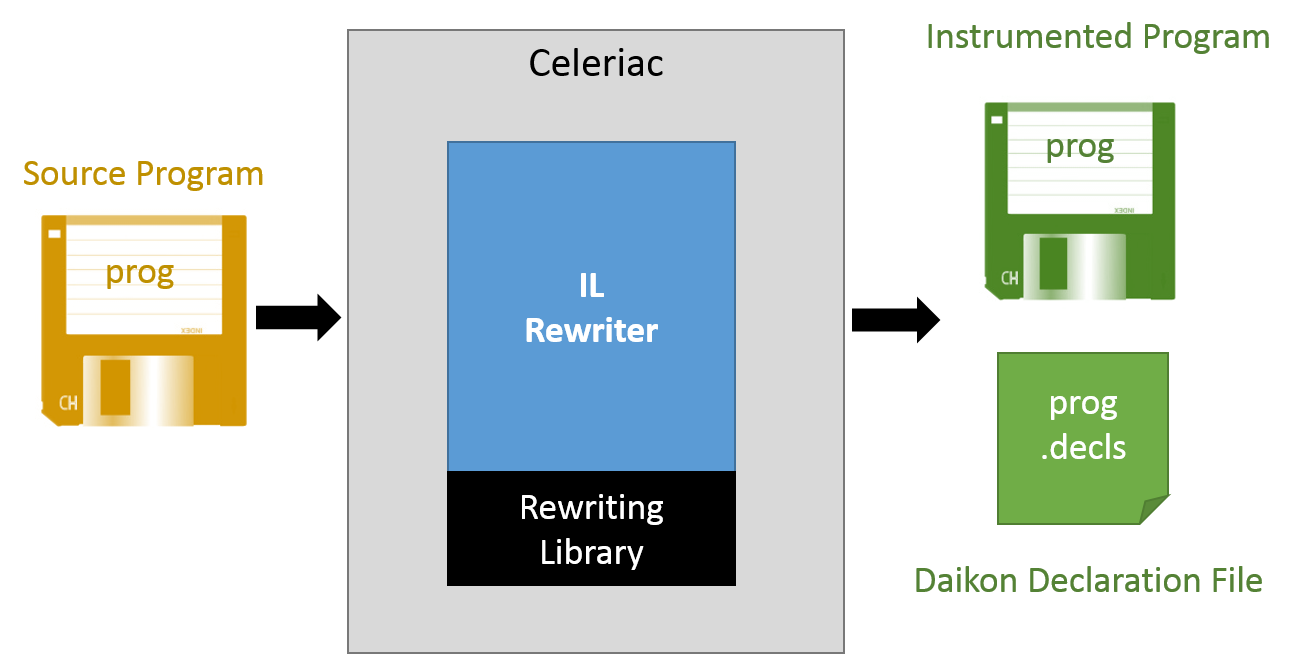
\includegraphics[scale=.7]{Arch1}
\end{center} \captionof{figure}{IL Rewriter Architecture}

A Daikon datatrace file consists of two parts. The first, called the declaration component, is metadata describing the schema of each program point (method entrance or exit).
While Celeriac is inserting instrumentation calls the IL rewriter also makes calls to the \texttt{DeclarationPrinter} class which writes the declaration portion of the datatrace file. The second component, the datatrace component, will be written by the program as it executes. When the IL rewriter is finished, it returns a memory stream which the front-end loads and executes, or saves to disk if desired.

\subsection{Runtime Library}
The runtime library creates the actual datatrace file that will be input to Daikon. The main method exposed to source programs prints the name of a variable, and its value, then prints the name and value of each of that variables fields, pure methods, and elements if any. The following figure illustrates the functionality of the runtime library component.

\begin{center}
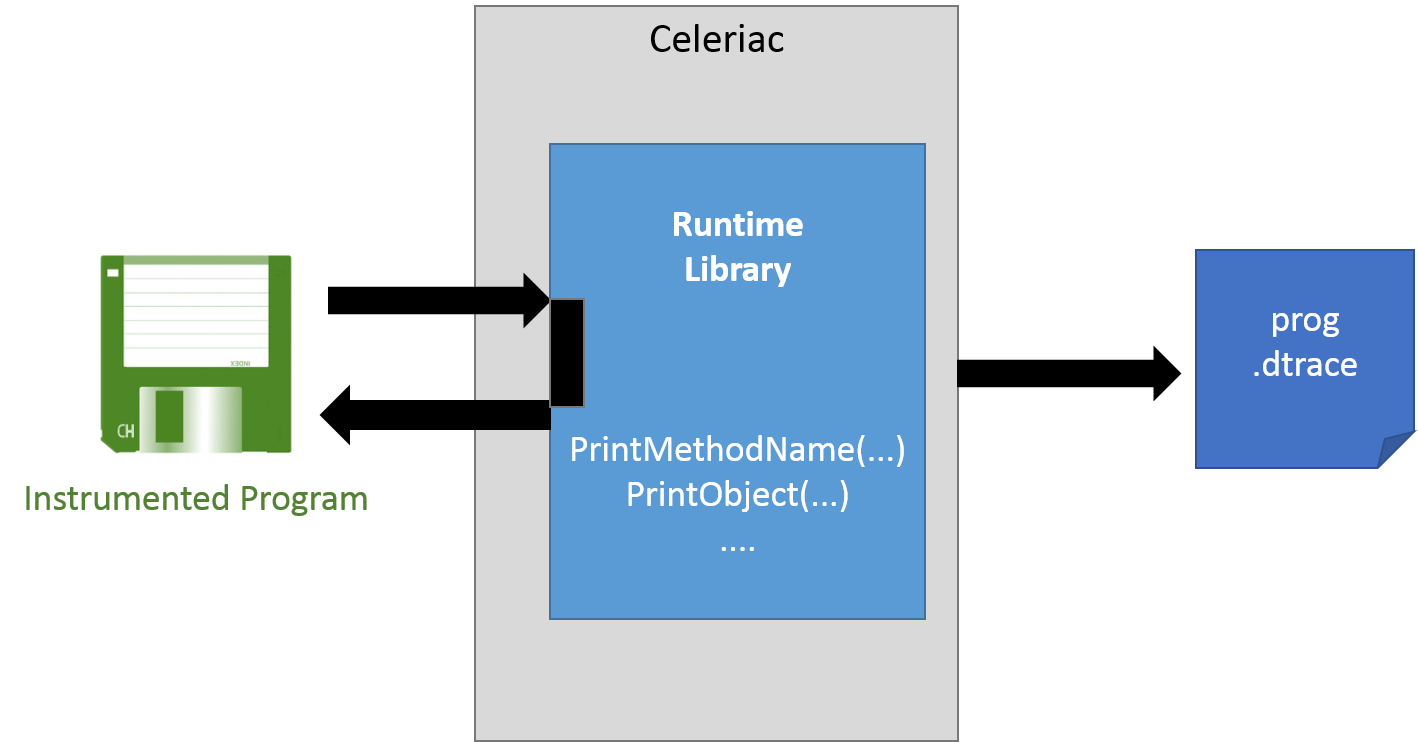
\includegraphics[scale=.7]{Arch2}
\end{center} \captionof{figure}{Runtime Library Architecture}
\~ \\

The runtime library is implemented in the \texttt{VariableVisitor} class. When the \texttt{VisitVariable()} method is called from the instrumented program the value of the variable itself is printed. Then any static or instance fields of that variable, which are visited reflectively based on the declared type of the variable are also printed. The instrumentation code traverses data structures and enumerates variables that implement the IList, ISet, or Dictionary interfaces, or their F\# equivalents.

%\section{Risks}
%This section describes the aspects of the project that are the riskiest, that is parts of the project may be difficult to complete during the fall (or at all).

%\paragraph{Instrumenting Exception Return Points}
%The instrumentation calls that the unmanaged profiler adds must maintain the validity of the MSIL code. For function prologues, this maintaining validity is apparently easy. For intermediary return points and exceptional return points, this is not trivial \cite{Mikunov:2003:Online}.

%\paragraph{Detecting / Instrumenting Complex Language Features}
%Certain language features, such a closures, may be compiled into weird
%constructs in the MSIL. It may be hard or impossible to detect all of
%these features in the MSIL code an instrument them accordingly.

\appendix

\section{Appendix: Project Schedule and Milestones}
This section describes the project milestones and history.

\subsection{10/2010 - 12/2010}
Work began on the instrumentor this quarter. A first attempt was to use the unmanaged Profiler API. First C\# reflection was used to analyze the program, and then the Profiler API's function enter/leave hooks were used to output the appropriate variable information. Manually editing the MSIL was extremely difficult and error-prone, especially for methods with multiple exit points and exception handling, so this approach was abandoned.

A pure IL rewriting approach using the CCIMetadata Library was attempted, where the output program was saved to disk as a new executable, however this violated the Disk Modifications Avoidance design goal. A hybrid of the previous two methods was considered where the CCIMetadata Library would create the new MSIL, and this would be handed to the unmanaged Profiler, to be substituted for the original method IL.

A presentation of the work to this point was presented to the UW CSE PL\&SE group on December 13th.
\subsection{1/2011 - 3/2011}
The previously described method was almost immediately shown to be infeasible. The CCIMetadata rewritten code produced different method tokens than were present in the original program, and thus could not be used. The main developer on the CCIMetadata project confirmed this issue could not be resolved in context. Analysis of alternate methods for IL rewriting was completed. It was determined that using the program with instrumentation inserted by CCIMetadata, but loaded into memory and ran instead of written to disk was the best approach.

The remainder of the quarter was spend implementing the profiler and visitor, and getting them to conform to Daikon specification. At the conclusion of the quarter an alpha version of the front end was functional, and could generate simple datatrace files that Daikon could process.

\subsection{4/2011 - 6/2011}
During this quarter reflective visiting and array-style visiting of IEnumerable types were implemented. Most command-line arguments available to Chicory were documented. A test suite was added, modeled off the Kavasir (C++) front-end test suite. Chicory test sources were transliterated from Java to C\# and ran through the front-end. Output invariants were compared to the invariants produced by Chicory, and bugs in the front-end were fixed to rectify the differences. Exception handling was also added, a feature new to Daikon front-ends.

\subsection{4/2012 - 6/2012}
\begin{comment}
\subsection{Introductory Milestones - From the 10/2010 - 12/2010 section}

\subsubsection{Read the First Three Sections of the Daikon User Manual}
Read the first three sections of the Daikon Developer Manual \cite{DaikonUserManual:Online}. Perform the Java \verb|StackAr| example to get an idea of what Daikon can do and what it is like to use Daikon.

\timetbl{10/4/2010}{2 hours}{10/5/2010}{2 hours}

\subsubsection{Read the ``New Front Ends'' Section of the Daikon Developer Manual}
Read the ``New Front Ends'' section of the Daikon Developer Manual \cite{DaikonDeveloperManual:Online}

\timetbl{10/6/2010}{1 hour}{10/6/2010}{1 hour}

\subsubsection{Read the File Formats Appendix}
Read the ``File Formats'' appendix of the Daikon Developer Manual to get a clearer idea of the information that the front end will have to output.

\timetbl{}{}{}{}

\subsubsection{Install Visual Studio 2010 Ultimate Edition from MSDNAA}
Download and install a copy of Visual Studio 2010 Ultimate Edition form the MSDNAA website. It is available for free. We have to use Visual Studio 2010 Ultimate Edition in order to use Microsoft Research's tools (e.g., the code contract framework).

\timetbl{10/6/2010}{1.5 hours}{10/6/2010}{1.5 hours}

\subsection{Profiler Milestones}

\subsubsection{Hello World}
Build an unmanaged profiler that logs "Hello World" to a file specified by the user via the command line whenever a program is run using the profiler.

\timetbl{10/17/2010}{7 hours}{10/17/2010}{8 hours}

\subsubsection{Function Names}
Modify the profiler to log the name of each function that is compiled by the JIT right before they are compiled.

\timetbl{10/25/2010}{15 hours}{}{}

\subsubsection{Function Names 2.0}
Modify the profiler to insert a prologue in each function that outputs the name of the function to the log whenever it is called.
We decided we didn't need to do a prologue after all.
\timetbl{}{}{}{}

\subsubsection{Parameter Names}
Modify the profiler to insert a prologue in each function that outputs the names of the function parameters to the log whenever it is called.
Didn't end up using a prologue, instead use reflection to output function parameter names to a file, then parse those in the profiler.
\timetbl{}{}{11/11/2010}{22 hours}

\subsection{Instrumentation Milestones}

This section was left intentionally blank
\end{comment}
\newpage
\bibliographystyle{plain}
\bibliography{daikon-dotnet}

\end{document}


